%auto-ignore
\providecommand{\MainFolder}{..}
\documentclass[\MainFolder/Text.tex]{subfiles}

\begin{document}

\section{Computation of Chern-Simons Maurer-Cartan element for spheres}
\allowdisplaybreaks
\label{Section:MCSphere}

We recall from Definition~\ref{Def:PushforwardMCdeRham} that the Chern-Simons Maurer-Cartan element~$\PMC$ is computed as a sum over trivalent ribbon graphs decorated with the admissible Hodge Propagator~$\Prpg$ at internal edges, integration variables $x_i$ at internal vertices and, in the case of $\Sph{n}$, with $\NOne$ or $\NVol$ at external vertices.
\begin{figure}[t]
\centering
%auto-ignore
\begin{tikzpicture}

\tikzset{point/.style = {draw, circle, fill=black, minimum size=2pt,inner sep=0pt}}

\def\dist{4}
\def\startangle{90}
\def\leglength{1.2}

\node[point,label={125:$x_1$}] (A) at (0,0) {};

\path[draw] (A) -- +(\startangle:\leglength) node[at end,right]{$\NVol$};
\path (A) -- +(\startangle:\leglength) node[point,style={fill=white}] {};
\path[draw] (A) -- +(\startangle+120:\leglength) node[at end, above, yshift=2pt]{$\NOne$};
\path (A) -- +(\startangle+120:\leglength) node[point,style={fill=white}] {};
\path[draw] (A) -- +(\startangle+240:\leglength) node[at end, above, yshift=2pt]{$\NOne$};
\path (A) -- +(\startangle+240:\leglength) node[point,style={fill=white}] {};

\end{tikzpicture}
\caption{The $Y$-graph for $\Sph{n}$.}\label{Fig:YGraph}
\end{figure}

The canonical Maurer-Cartan element $\MC$ is the contribution of the Y-graph (see Figure~\ref{Fig:YGraph}), and it is easy to see that
\begin{equation*}
 \MC_{10}(\Susp \NVol \NOne \NOne ) = (-1)^n \MC_{10}(\Susp\NOne \NVol \NOne) = \MC_{10}(\Susp \NOne \NOne \NVol) = (-1)^{n-2}.
\end{equation*}
%We fix an input $\omega_1$, $\dotsc$, $\omega_l \in \BCyc\Harm(\Sph{n})$ of $\PMC_{lg}$ and let $\Gamma \in $ be an admissible trivalent ribbon graph with $e\ge 1$. We let $L$ be an admissible labeling of $\Gamma$.
%$\Gamma \in \TRRG_{klg}$ with the input $\omega_1$, $\dotsc$, $\omega_l$
Throughout this section, we will be in the setting of Definition~\ref{Def:PushforwardMCdeRham}.
In particular, $\Gamma \in \TRG_{klg}$ is a ribbon graph, $L$ its compatible labeling admissible with respect to an input $\omega_1$, $\dotsc$, $\omega_l$ and $I(\sigma_L)$ the corresponding integral.
\begin{Lemma}[Condition $(V_{\NOne})$ holds] \label{Lemma:ABVanishing}
For the Hodge Propagator $\Prpg$ from~\eqref{Eq:GreenKernelMC1} for $\Sph{n}$ for $n\ge 1$, every graph $\Gamma \neq Y$ with~$\NOne$ at an external vertex vanishes.
\end{Lemma}
\begin{proof}
%Before we begin appeal to~\cite{Cieliebak2018} for the fact that the integrand of $I(\sigma_L)$ is $L^1$-integrable, so that we can apply Fubini's theorem and integrate out a single vertex.
The only contribution of an $A$-vertex which does not vanish for degree reasons is
\[ A_{\NVol,\NOne}(y) = \int_x \Prpg(x,y) \Vol(x). \]
From the symmetry of $\Prpg$ and $\Vol$ under the action of $O(n+1)$, we get
\[ R^* A_{\NVol, \NOne} = (-1)^R A_{\NVol, \NOne}\quad\text{for all }R\in O(n+1). \]
Therefore, it suffices to check that $A_{\NVol, \NOne}(\StdBasis_1) = 0$, where $\StdBasis_1$, $\dotsc$, $\StdBasis_{n+1}$ denotes the standard basis of $\R^{n+1}$.
Evaluation of~\eqref{Eq:FormOmega1} at $(x,\StdBasis_1)$ gives
\[ \omega_0(x,\StdBasis_1) = \frac{1}{(n-1)!} \sum_{\substack{\sigma\in\Perm_{n+1}\\ \sigma_2 = 1}} (-1)^\sigma x^{\sigma_1} \Diff{y^{\sigma_3}} \dotsm \Diff{y^{\sigma_{n+1}}}. \]
%\marginnote{Can I argue more geometrically without integrating out one variable?}
Therefore, we get
\begin{align*}
A_{\NVol, \NOne}(\StdBasis_1) &= (-1)^n \int_x g_0(x\cdot \StdBasis_1) \omega_0(x,\StdBasis_1) \Vol(x)  \\ 
&= (-1)^{n+1} \int_x g_0(x^1) \Bigl( \sum_{j=2}^{n+1} (-1)^{j} x^j\Bigr) \Vol(x) \Diff{y^2} \dotsm  \widehat{\Diff{y^j}} \dotsm \Diff{y^{n+1}},
\end{align*}
where we view $g_0$ as a function of $x\cdot y$.
Consider the cyclic permutation of $x^2$, $\dotsc$, $x^{n+1}$:
\begin{align*} 
I:\Sph{n} &\longrightarrow \Sph{n} \\
   (x^1, x^2, \dotsc, x^n, x^{n+1}) &\longmapsto (x^1, x^{n+1}, x^2 \dotsc, x^{n}). 
\end{align*}
Then we have
\begin{align*}
\int_x g_0(x^1) \sum_{j=2}^{n+1} (-1)^{j} x^j \Vol(x)  &= (-1)^{n-1}\int_x I^*\Bigl(g_0(x^1) \sum_{j=2}^{n+1} (-1)^{j} x^j \Vol(x)\Bigr) \\
& = (-1)^{n-1} \int_x g_0(x^1)\Bigl(-\sum_{j=2}^{n+1} (-1)^j x^j\Bigr)\bigl((-1)^{n-1}\Vol(x)\bigr) \\
& = - \int_x g_0(x^1) \sum_{j=2}^{n+1} (-1)^{j} x^j \Vol(x).
\end{align*}
It follows that $A_{\NVol,\NOne}(\StdBasis_1)=0$.\footnote{Notice that we avoided using $\sum \int = \int \sum$ because the convergence of single summands is not guaranteed.}

Let us now consider the contribution of a $B$-vertex with $\NOne$:
%\marginnote{In order to prove rotational symmetry of $\eta_B^{\NOne}$ rigorously, I have to lift the action to the double blowup. Can it be argued without blowing up?}
\[ B_{\NOne}(y,z) = \int_{x} \Prpg(y,x) \Prpg(x,z) = (-1)^n \int_x \Prpg(y,x) \Prpg(x,z). \]
For $n=1$, the degree of $\Prpg(y,x)\Prpg(x,z)$ is $0$, and hence $B_{\NOne}= 0$ trivially.
Suppose that $n\ge 2$.
As in the case of $A_{\NVol,\NOne}$, we get that 
\[ R^* B_{\NOne} = (-1)^R B_{\NOne} \quad\text{for all }R\in O(n+1). \]
Therefore, it suffices to check that $B_{\NOne}(\StdBasis_1, c_1 \StdBasis_1 + c_2 \StdBasis_2) = 0$ for all $(c_1,c_2)\in \Sph{1}$.
We have
\[  B_{\NOne}(\StdBasis_1, c_1 \StdBasis_1 + c_2 \StdBasis_2) = \begin{multlined}[t] (-1)^n \int_x \sum_{a=1}^{n-1} g_a(x^1) g_{n-a}(c_1 x^1 + c_2 x^2)\omega_a(x,\StdBasis_1) \\ \omega_{n-a}(x,c_1 \StdBasis_1 + c_2 \StdBasis_2).\end{multlined}\]
We will show that for every $a=1$,~$\dotsc$, $n-1$ we can write
\begin{equation} \label{Eq:Mu}
\mu_a(x) \coloneqq \omega_a(x,\StdBasis_1) \omega_{n-a}(x,c_1 \StdBasis_1 + c_1 \StdBasis_2) = \Bigl(\sum_{i=3}^{n+1} \pm  x^i \Vol(x)\Bigr) \eta_a(y,z)
\end{equation}
with alternating signs for some form $\eta_a(y,z)$.
Then we can use the same argument as for~$A_{\NVol,\NOne}$ with the cyclic permutation of $x^3$, $\dotsc$, $x^{n+1}$ given by
\begin{align*} 
I':\Sph{n} &\longrightarrow \Sph{n} \\
   (x^1, x^2, x^3,\dotsc, x^n, x^{n+1}) &\longmapsto (x^1, x^2, x^{n+1}, x^3 \dotsc, x^{n}) 
\end{align*}
%\begin{align*}
%& \int_x  g_a(x^1) g_{n-a}(c_1 x^1 + c_2 x^2) x^i \Vol(x) \\
%&\qquad = - \int_x I^*_i \bigl(g_a(x^1) g_{n-a}(c_1 x^1 + c_2 x^2) x^i \Vol(x)\bigr) \\
%&\qquad = - \int_x g_a(x^1) g_{n-a}(c_1 x^1 + c_2 x^2) (-x^i) (-\Vol(x))
%\end{align*}
%for all $3 \le i \le n+ 1$, and hence
to conclude that $B_{\NOne}(\StdBasis_1, c_1 \StdBasis_1 + c_2 \StdBasis_2) = 0$.

In order to show \eqref{Eq:Mu}, we have to study the product of $\omega_i$'s.
From~\eqref{Eq:FormOmega1} we get
\begin{equation}\label{Eq:GenProd}
\begin{aligned}
&\omega_a(x,y)\omega_{n-a}(x,z)\\
&\quad =\begin{multlined}[t] \frac{1}{a! (n-1-a)! (n-a)! (a-1)!} \sum_{\substack{\sigma,\,\mu\in \Perm_{n+1}}} (-1)^{\sigma + \mu} x^{\sigma_1} x^{\mu_1} y^{\sigma_2} z^{\mu_2}  \\ \Diff{x}^{\sigma_3} \dotsm \Diff{x}^{\sigma_{2+a}} \Diff{x}^{\mu_3}\dotsm\Diff{x}^{\mu_{2+n-a}} 
\Diff{y}^{\sigma_{3+a}}\dotsm \Diff{y}^{\sigma_{n+1}}\\\Diff{z}^{\mu_{3+n-a}}\dotsm \Diff{z}^{\mu_{n+1}}.
\end{multlined}
\end{aligned}
\end{equation}
In order to simplify this expression, we decompose $\sigma\in \Perm_{n+1}$ as
\begin{equation} \label{Eq:Decomp}
 \sigma = \sigma^5 \circ \sigma^4 \circ \sigma^3 \circ \sigma^2 \circ \sigma^1,
 \end{equation}
where $\sigma^1$, $\dotsc$, $\sigma^5\in \Perm_{n+1}$ are permutations defined as follows:
\begin{itemize}
 \item The permutation $\sigma^1$ is a shuffle permutation $\sigma^1 \in \Perm_{2+a,n-a-1}$ such that its first block denoted by $\sigma^1(1) = (\sigma^1_1,\dotsc,\sigma^1_{2+a})$ is equal to the ordered set $\{\sigma_1, \dotsc, \sigma_{2+a}\}$.
 The second block $\sigma^1(2)$ is then the ordered set $\{\sigma_{3+a},\dotsc,\sigma_{n+1}\}$, which will be denoted by $J_\sigma$.
 \item The permutation $\sigma^2$ acts on the block $\sigma^1(1)$ by moving $\sigma_2$ in front.
 We denote the new block $\sigma^1(1)\backslash\{\sigma_2\}$ by $I_\sigma$, so that we can write $\sigma^2 : \sigma^1(1) \mapsto (\sigma_2, I_\sigma)$. 
 \item The permutation $\sigma^3$ acts on the block $I_\sigma$ by moving $\sigma_1$ in front.
 Together with the previous step we get $\sigma^1(1)\mapsto (\sigma_2, \sigma_1,I_\sigma\backslash\{\sigma_1\})$.
 \item The permutation $\sigma^4$ is a transposition of $\sigma_1$ and $\sigma_2$.
 \item The permutation $\sigma^5$ is determined by the pair $(\sigma^{51},\sigma^{52}) \in \Perm_{a} \times \Perm_{n-1-a}$ of permutations $\sigma^{51}$ and $\sigma^{52}$ acting on blocks $I_\sigma\backslash\{\sigma_1\}$ and $J_\sigma$ to get $(\sigma_3,\dotsc,\sigma_{2+a})$ and $(\sigma_{3+a},\dotsc,\sigma_{n+1})$, respectively.
\end{itemize}



We define the decomposition $\mu^1$,~$\dotsc$, $\mu^5$ for $\mu\in \Perm_{n+1}$ from \eqref{Eq:GenProd} analogously with $a$ replaced by $n-a$.
Using~\eqref{Eq:Decomp}, the product~\eqref{Eq:GenProd} can be written as
\begin{align*}
  &\begin{multlined}\frac{1}{a! (n-1-a)! (n-a)! (a-1)!} \sum_{\substack{\sigma^1,  \dotsc,\, \sigma^5 \\ \mu^1, \dotsc,\, \mu^5}} (-1)^{\sigma^1 + \dotsb + \sigma^5 + \mu^1 + \dotsb + \mu^5} x^{\sigma_1} x^{\mu_1} y^{\sigma_2} z^{\mu_2} \\ \Diff{x}^{\sigma^{51}(I_\sigma\backslash \{\sigma_1\})} \Diff{x}^{\mu^{51}(I_\mu\backslash\{\mu_1\})} \Diff{y}^{\sigma^{52}(J_\sigma)} \Diff{z}^{\mu^{52}(J_\mu)} \end{multlined} \\[5pt]
 &\qquad =\begin{multlined}[t]- \sum_{\sigma^1,\, \mu^1} (-1)^{\sigma^1 + \mu^1} \Bigl(\sum_{\sigma^2,\, \mu^2} (-1)^{\sigma^2 + \mu^2} \sum_{\sigma^3,\, \mu^3} (-1)^{\sigma^3 + \mu^3} x^{\sigma_1} x^{\mu_1} y^{\sigma_2} z^{\mu_2} \\ \Diff{x}^{I_\sigma \backslash \{\sigma_1\}} \Diff{x}^{I_\mu\backslash \{\mu_1\}}\Bigr) \Diff{y}^{J_\sigma} \Diff{z}^{J_\mu},\end{multlined} \end{align*}
where $-1$ comes from $(-1)^{\sigma^4}$ and $\sigma^5$ is compensated by permutations of forms.
For fixed $\sigma^1$ and $\mu^1$, consider the coefficient at $\Diff{y}^{J_\sigma}\Diff{z}^{J_\mu}$ in the brackets.
If we evaluate it at $y=\StdBasis_1$, $z=c_1 \StdBasis_1 + c_2 \StdBasis_2$, we get
\begin{align*}
&  c_1 \overbrace{\sum_{\substack{\sigma^3,\, \mu^3 \\ \sigma_2 = 1 \\ \mu_2 = 1}} (-1)^{\sigma^3 + \mu^3} x^{\sigma_1} x^{\mu_1}  \Diff{x}^{I_\sigma\backslash\{\sigma_1\}} \Diff{x}^{I_\mu \backslash\{\mu_1\}}}^{=:\displaystyle\mathrm{I}} \\ 
& {} + (-1)^{\mu^2} c_2  \overbrace{\sum_{\substack{\sigma^3,\, \mu^3 \\ \sigma_2 = 1 \\ \mu_2 = 2}} (-1)^{\sigma^3 + \mu^3} x^{\sigma_1} x^{\mu_1}  \Diff{x}^{I_\sigma\backslash\{\sigma_1\}} \Diff{x}^{I_\mu \backslash\{\mu_1\}}}^{=:\displaystyle\mathrm{II}},
 \end{align*}
where $(-1)^{\mu^2} = -1$ if and only if $1\in I_{\mu}$.

More generally, for multiindices $I_1$, $I_2 \subset \{1,\dotsc, n+1\}$ of lengths $a+1$ and $n-a+1$,  respectively, consider the sum
\begin{equation} \label{Eq:Sum}
S(I_1,I_2) \coloneqq \sum_{\substack{i_1 \in I_1 \\ i_2 \in I_2}} (-1)^{(i_1,I_1) + (i_2,I_2)} x^{i_1} x^{i_2} \Diff{x}^{I_1\backslash\{i_1\}} \Diff{x}^{I_2\backslash\{i_2\}},
\end{equation}
where $(i_j, I_j)$ is the number of transpositions required to move $i_j$ in front of $I_j$.
The following implication holds: 
\begin{equation*}
 S(I_1, I_2)\neq 0\; \Implies \; 1 \le \Abs{I_1 \cap I_2} \le 2.
\end{equation*}
We distinguish the two cases left: 
\begin{description}[font=\normalfont\itshape]
\item[Case $I_1 \cap I_2 =\{i,j\}$ with $i < j$: ] We get
\begin{align*} 
S(I_1, I_2) &= \begin{multlined}[t] (-1)^{(i,I_1) + (j,I_2)} x^{i} x^j \Diff{x}^{I_1 \backslash\{i\}} \Diff{x}^{I_2 \backslash \{j\}} \\ {}+ (-1)^{(j,I_1) + (i,I_2)} x^{j} x^i \Diff{x}^{I_1 \backslash\{j\}} \Diff{x}^{I_2 \backslash \{i\}} \end{multlined} \\
&=\begin{multlined}[t] (-1)^{(i,I_1) + (j,I_2) + (j,I_1)+1 + (i,I_2)} x^i x^j \Diff{x}^j \Diff{x}^{I_1\backslash\{i,j\}}\\\Diff{x}^i \Diff{x}^{I_2\backslash\{i,j\}} + (-1)^{(j,I_1) + (i,I_2)+(i,I_1)+ (j,I_2)+1} x^i x^j \\ \Diff{x}^i \Diff{x}^{I_1\backslash\{i,j\}}\Diff{x}^j \Diff{x}^{I_2\backslash\{i,j\}} \end{multlined} \\
&= \pm(-1 +  1) x^i x^j \Diff{x}^i \Diff{x}^{I_1\backslash\{i,j\}} \Diff{x}^j\Diff{x}^{I_2\backslash\{i,j\}},
\end{align*}
where in the last step we switched $\Diff{x}^i \leftrightarrow \Diff{x}^j$ in the first summand.
Therefore, it holds $S(I_1, I_2) = 0$.
\item[Case $I_1 \cap I_2 = \{i\}$:] We must have $I_1 \cup I_2 = \{1,\dotsc,n+1\}$.
A non-zero summand in~\eqref{Eq:Sum} has either $i_1 = i$ and $i_2\in I_2$, in which case \[I_1\backslash \{i_1\} \cup I_2\backslash\{i_2\}= \{1, \dotsc, \widehat{i_2}, \dotsc, n+1\}, \] or $i_2 = i$ and $i_1\in I_1$ with $i_1 \neq i$, in which case \[I_1\backslash \{i_1\} \cup I_2\backslash\{i_2\}= \{1, \dotsc, \widehat{i_1}, \dotsc, n+1\}.\] Indices $i_2$ from the first case and $i_1$ from the second case constitute $\{1,\dotsc,n+1\}$.
Therefore, for some signs $\pm$, we can write
\begin{equation*} \label{Eq:AlternatingSum}
S(I_1,I_2) = x^i \sum_{j=1}^{n+1}  \pm  x^j \Diff{x^1} \dotsm \widehat{\Diff{x^j}} \dotsm \Diff{x^{n+1}}.
\end{equation*}
%
We will prove that the signs alternate, and hence $S(I_1,I_2)= \pm x^i \Vol(x)$.
Suppose that $j$, $j+1 \in I_{1}$ for some $j\in \{1,\ldots,n\}$.
The two summands in~\eqref{Eq:Sum} with $(i_1, i_2)=(j, i)$ and $(i_1, i_2)= (j+1,i)$, respectively, give
\begin{align*}
& \begin{multlined}[t](-1)^{(j,I_1) + (i,I_2)} x^{j} x^{i} \Diff{x}^{I_1\backslash\{j\}} \Diff{x}^{I_2\backslash\{i\}} + (-1)^{(j+1,I_1) + (i,I_2)} x^{j+1} x^{i} \\ \Diff{x}^{I_1\backslash\{j+1\}}\Diff{x}^{I_2\backslash\{i\}} \end{multlined}
\\ &\quad= \begin{multlined}[t] (-1)^{(i,I_2)} x^{j} x^{i} \Diff{x}^{j+1}\Diff{x}^{I_1\backslash\{j, j+1\}} \Diff{x}^{I_2\backslash\{i\}}  \\ {}+ (-1)^{1 + (i,I_2)} x^{j+1} x^{i} \Diff{x}^j \Diff{x}^{I_1\backslash\{j, j+1\}} \Diff{x}^{I_2\backslash\{i\}} \end{multlined} \\
&\quad = (-1)^{(i,I_2)}x^i (x^j \Diff{x}^{j+1} - x^{j+1} \Diff{x}^j) \Diff{x}^{I_1\backslash\{j, j+1\}} \Diff{x}^{I_2\backslash\{i\}}.
\end{align*}
The signs clearly alternate.
A symmetric argument holds when $j$, $j+1\in I_2$.
Now assume that $j \in I_1$ and $j+1\in I_2$.
The two summands in~\eqref{Eq:Sum} which have $(i_1, i_2)=(j,i)$ and $(i_1, i_2) = (i,j+1)$, respectively, give
\begin{align*}
& \begin{multlined}[t] (-1)^{(j,I_1)+(i,I_2)} x^j x^i \Diff{x}^{I_1\backslash\{j\}}\Diff{x}^{I_2\backslash\{i\}} + (-1)^{(i,I_1) + (j+1,I_2)} x^i x^{j+1} \\ \Diff{x}^{I_1\backslash\{i\}}\Diff{x}^{I_2\backslash\{j+1\}} \end{multlined}\\
&\quad=\begin{multlined}[t]
(-1)^{(j,I_1)+(i,I_1\backslash\{j\}) + (a + 1)} x^j x^i \Diff{x^{I_1\backslash\{i, j\}}}\Diff{x}^{I_2} \\ {}+ (-1)^{(i,I_1) + (j+1,I_2) + (j,I_1\backslash\{i\})} x^i x^{j+1} \Diff{x}^j \Diff{x}^{I_1\backslash\{i, j\}} \Diff{x}^{I_2\backslash\{j+1\}}
\end{multlined}\\&\quad=
\begin{multlined}[t]
(-1)^{(j,I_1) + (i,I_1\backslash\{j\})+(j+1,I_2)} x^i x^j \Diff{x}^{j+1} \Diff{x}^{I_1\backslash\{i,j\}} \Diff{x}^{I_2\backslash\{j+1\}} \\ {}+ (-1)^{1 + (j,I_1) + (i,I_1\backslash\{j\})+(j+1,I_2)} x^i x^{j+1} \Diff{x}^j \Diff{x}^{I_1\backslash\{i,j\}} \Diff{x}^{I_2\backslash\{j+1\}} 
\end{multlined}\\
&\quad= \begin{multlined}[t] (-1)^{(j,I_1) + (i,I_1\backslash\{j\})+(j+1,I_2)} x^i (x^j \Diff{x}^{j+1} - x^{j+1} \Diff{x}^j) \\ \Diff{x}^{I_1\backslash\{i,j\}} \Diff{x}^{I_2\backslash\{j+1\}}. \end{multlined}
\end{align*}
The signs alternate again.
A symmetric argument holds for $j\in I_2$ and $j+1\in I_1$.
\end{description}	 

 Back to the original problem, we have $\mathrm{I} = S(I_\sigma, I_\mu)$ with $I_\sigma, I_\mu \subset \{2,\dotsc, n+1\}$.
 It follows that the first case applies, and hence $\mathrm{I} = 0$. 
 We have $\mathrm{II} = S(I_\sigma, I_\mu)$ with $I_\sigma \subset \{2,\dotsc, n+1\}$ and $I_\mu \subset \{1, \widehat{2}, \dotsc, n+1\}$.
 It follows that either the first case or the second case with $i\ge 3$ applies.
 This proves~\eqref{Eq:Mu} up to signs.
 Tracing back the signs, one can convince himself that the signs in \eqref{Eq:Mu} indeed alternate.

The last paragraph of the proof of Proposition~\ref{Prop:COne} finishes the proof.
\end{proof}

We summarize the consequences in the following proposition.
The main argument is the same as in the proof of Proposition~\eqref{Prop:GeomForm}.

\begin{Proposition}[Vanishing of graphs for $\Sph{n}$] \label{Prop:TotalVanishing}
Consider $\Sph{n}$ with the Hodge Propagator~\eqref{Eq:GreenKernelMC1}.
Only the following trivalent ribbon graphs $\Gamma \neq Y$ do not necessarily vanish:
\begin{description}[font=\normalfont\itshape]
 \item[($n=1$):] The $O_{k}$-graph with $k\in 2\N$ internal vertices of type $B$ with $\NVol$ at the external vertex (see Figure~\ref{Fig:Gamma0}).
 \item[($n=2$):] It must hold $A=0$, $C=2B$ and all $B$ vertices must have $\NVol$ at the external vertex.
 Moreover, if $\Gamma$ is reduced, it must have $g\ge 1$.
 \item[($n=3$):] There is no external vertex and $4 \mid C$ holds.
 \item[($n>3$):] All graphs vanish.
\end{description}
%The conclusion is that $\PMC_{10} = \MC_{10}$ and $\PMC_{klg} = 0$ for $(l,g) \ne (1,0)$ in any dimension $n$ with the possible exception of $\PMC_{20}$ for $n=1$ and $\PMC_{lg}$ with $g\ge 1$ for $n=2$.
\end{Proposition}
\begin{proof}
%Thanks to Lemma~\ref{Lemma:ABVanishing}, we can apply  Proposition~\ref{Prop:PMCEqualsMC} to get $\PMC_{10} = \MC_{10}$, $\PMC_{20} = 0$ for $n \ge 2$ as $H_{\mathrm{dR}}^1(\Sph{n}) = 0$, and $\PMC_{lg} = 0$ for all $(l,g)\neq (1,0)$, $(2,0)$ for $n>3$.
Lemma~\ref{Lemma:ABVanishing} implies that $A=0$ and that the total form-degree $D$ satisfies $D= n B$.
Therefore, we get from \eqref{Eq:VerticesEq} the following: for $n>3$ there is neither a $B$-vertex nor a $C$-vertex; for $n=3$, there is no $B$-vertex; for $n=2$, we have $C=2B$; and for $n=1$, there is no $C$-vertex.

Consider the pullback of $I(\sigma_L)$ along the (multi)diagonal action of an $R\in O(n+1)$ with $\Det(R)=-1$ on $(\Sph{n})^{\times k}$.
We get schematically
\[ \int_{(\Sph{n})^{\times k}} \Prpg^{e}\Vol^{s} = (-1)^{k +e + s} \int_{(\Sph{n})^{\times k}} G^{e}\Vol^{s}. \]
Therefore, $k+ e + s$ has to be even.
If we plug-in from~\eqref{Eq:ChangeOfVariables}, we get
\[ k+ e + s =  \begin{cases}
3 B & \text{for }n=1, \\
8 B & \text{for }n=2, \\
\frac{5}{2} C & \text{for }n=3.
\end{cases} \]

A non-vanishing reduced graph must have $B\ge l$.
For $n=2$, so that $C=2B$, the formula~\eqref{Eq:GenusFormulaa} gives $g\ge 1$.
\end{proof}

\begin{Remark}[Graphs for $\Sph{2}$]\phantomsection\label{Rem:GraphsTwoSphere}

{ \begingroup
\begin{figure}
\centering
\begin{subfigure}{0.45\textwidth}
\centering
%auto-ignore
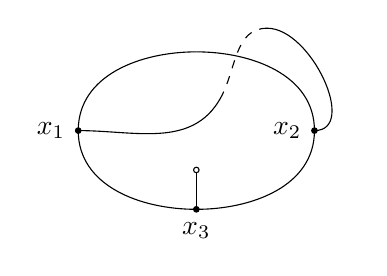
\begin{tikzpicture}
 \tikzset{point/.style = {draw, circle, fill=black, minimum size=2pt,inner sep=0pt}}
 \tikzset{->-/.style={decoration={markings,mark=at position #1 with {\arrow{>}}},postaction={decorate}}}
 
 \def\lenI{3cm}
 \def\lenII{1cm}
 \def\lenext{0.5cm}
 
 \coordinate (x1) at (0,0) {};
 \coordinate (x2) at (\lenI,0);
 \coordinate (x3) at (0.5*\lenI,-1*\lenII);

 \coordinate (p4) at (0.5*\lenI,\lenII);
 \coordinate (p5) at (0.6*\lenI,0.4*\lenII);
 \coordinate (p6) at (0.8*\lenI,1.3*\lenII);

 \draw (x1) to[out=90,in=180] (p4);
 \draw (p4) to[out=0,in=90] (x2);
 \draw (x1) to[out=-90,in=180] (x3);
 \draw (x3) to[out=0,in=-90] (x2);
 \draw (x1) to[out=0,in=-120] (p5);
 \draw[dashed] (p5) to[out=60,in=180] (p6);
 \draw (p6) to[out=0,in=0] (x2);
 
 \node[point,label={180:$x_1$}] at (x1) {};
 \node[point,label={180:$x_2$}] at (x2) {};
 \node[point,label={-90:$x_3$}] at (x3) {};
 
 \draw (x3) -- +(90:\lenext) node[point,,style={fill=white},label={180:$\NVol$}] {};
\end{tikzpicture}
\caption{$P_1$}
\end{subfigure}
\begin{subfigure}{0.45\textwidth}
\centering
%auto-ignore
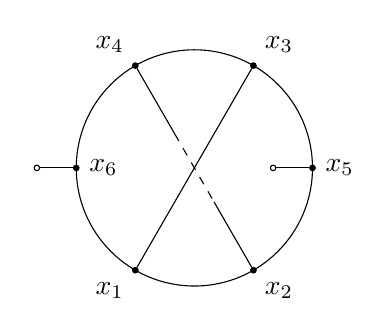
\begin{tikzpicture}
 \tikzset{point/.style = {draw, circle, fill=black, minimum size=2pt,inner sep=0pt}}
 \tikzset{->-/.style={decoration={markings,mark=at position #1 with {\arrow{>}}},postaction={decorate}}}
 
 \def\rad{1.5cm}
 \def\ang{60}
 \def\dashsep{0.5cm}
 \def\lenext{0.5cm}
 
 \coordinate (C) at (0,0);
 \draw (C) circle (\rad);

 \path (C) node[point,label={0:$x_5$}] (x5)  at +(0*\ang:\rad){};
 \path (C) node[point,label={\ang:$x_3$}] (x3)  at +(1*\ang:\rad){};
 \path (C) node[point,label={2*\ang:$x_4$}] (x4)  at +(2*\ang:\rad){};
 \path (C) node[point,label={0:$x_6$}] (x6)  at +(3*\ang:\rad){};
 \path (C) node[point,label={4*\ang:$x_1$}] (x1)  at +(4*\ang:\rad){};
 \path (C) node[point,label={5*\ang:$x_2$}] (x2)  at +(5*\ang:\rad){};
 
 \draw (x5) -- +(180:\lenext) node[point,style={fill=white},label={90:$\NVol$}] {};
 \draw (x6) -- +(180:\lenext) node[point,style={fill=white},label={90:$\NVol$}] {};
 \draw (x1) -- (x3);
 
 \path (C) coordinate (p1)  at +(2*\ang:\dashsep){};
 \path (C) coordinate (p2)  at +(-1*\ang:\dashsep){};
 
 \draw (x2) -- (p2);
 \draw (x4) -- (p1);
 \draw[dashed] (p1) -- (p2);
\end{tikzpicture}
\caption{$P_2$}
\end{subfigure}
\caption{Vanishing graphs $P_1$ and $P_2$ for $\Sph{2}$.}\label{Fig:P1P2}
\end{figure}
\endgroup }
The simplest possibly non-vanishing graph for $\Sph{2}$ has $A= 0$, $B=1$, $C=2$. If it is reduced, we must have $l = g = 1$, and hence it will contribute to $\PMC_{11}$. Up to an isomorphism, there is only one such graph, which we denote by $P_1$ (see Figure~\ref{Fig:P1P2}). However, we see that the pair of internal vertices $x_1$ and $x_2$ is connected by two edges, which implies that $P_1 =0$. Indeed, $\Prpg(x,y)$ has odd degree, and hence we have\footnote{We recall from Section~\ref{Section:Proof2} that the notation $\Prpg(x_i,x_j)$ means $(\pi_{i} \times \pi_j)^* \Prpg$ and not just the evaluation at $(x_i,x_j)$.}
\[ \Prpg(x,y)\Prpg(y,x) = \Prpg(x,y)^2 = 0 \]
by the symmetry on the pullback along the twist map. It follows that $\PMC_{11} = 0$.

The second simplest possibly non-vanishing reduced graph is the graph~$P_2$ from Figure~\ref{Fig:P1P2}. Let 
\begin{equation*}
\eta(x_1,x_2,x_3,x_4,x_5) \coloneqq\begin{multlined}[t]\Prpg(x_1,x_2)\Prpg(x_1,x_3)\Prpg(x_4,x_2)\Prpg(x_4,x_3)\Prpg(x_3,x_5)\\ \Prpg(x_2,x_5)\Vol(x_5) \end{multlined}
\end{equation*}
denote the form in the integrand coming from the part of the graph on the right-hand side of the vertical axis going through $x_1$, $x_4$. If $\tau_{1,4}$ denotes the exchange of $x_1$ and $x_4$, then clearly $\tau_{1,4}^* \eta = \eta$ because the graph is symmetric with respect to the horizontal axis going through $x_5$, $x_6$. Using this, we compute
\begin{align*}
& \int_{x_1,x_2,x_3,x_4,x_5,x_6} \NVol(x_6)\Prpg(x_1,x_6)\Prpg(x_4,x_6) \eta(x_1,x_2,x_3,x_4,x_5) \\
& = \int_{\tau_{1,4}(x_1,x_2,x_3,x_4,x_5,x_6)} \tau_{1,4}^*\bigl(\NVol(x_6)\Prpg(x_1,x_6)\Prpg(x_4,x_6) \eta(x_1,x_2,x_3,x_4,x_5)\bigr) \\
& = \int_{x_4,x_2,x_3,x_1,x_5,x_6} \NVol(x_6)\Prpg(x_4,x_6)\Prpg(x_1,x_6) \eta(x_4,x_2,x_3,x_1,x_5)\\
& = 
 -\int_{x_1,x_2,x_3,x_4,x_5,x_6} \NVol(x_6)\Prpg(x_1,x_6)\Prpg(x_4,x_6)  \eta(x_1,x_2,x_3,x_4,x_5),
\end{align*}
where the minus sign comes from switching the first two $\Prpg$'s. We see that $P_2$ vanishes. The other variants with $x_5$ moved on the edge $x_3$, $x_4$ and~$x_2$, $x_4$ vanish by a similar argument using the compositions $\tau_{1,3}\circ\tau_{5,6}$ and $\tau_{1,2}\circ\tau_{5,6}$, respectively. We conclude that $\PMC_{21} = 0$, and hence $\OPQ_{121}^\PMC = 0$. 

We sum up some general observations about the integrals for $\Sph{2}$:

\begin{itemize}
\item We have $B_{\NOne} \neq 0$ and $C \neq 0$ for the corresponding forms.
\item We have the multiplication formula (c.f., Example~\ref{Example:Circle})
\[ \omega_1(x,y) \omega_1(x,z) = x\cdot(y\times z) \Vol(x). \]
\item The number $(-1)^{\sigma_L} I(\sigma_L)$ does not depend on the choice of $L_1$ provided a compatible $L_2$ is chosen.
\item It holds $\sum_{L_3^b} (-1)^{\sigma_L} I(\sigma_L) = 0$ whenever there is a boundary component with even number of $\NVol$'s.
\item If there is a $B$-vertex $x$ such that the underlying graph (after forgetting the ribbon structure) is symmetric on the reflection along an axis going through $x$, then $I(\sigma_L) = 0$. \qedhere
\end{itemize}
% Because of \eqref{Eq:NonVanishingOf}, we think that an argument for vanishing of $I(\sigma_L)$ can not be local as in the proof of Lemma~\ref{Lemma:ABVanishing} but must use the graph structure in some way.

\Correct[caption={DONE Nonsense about lower bound}]{$g\ge 1$ is equivalent to $B \ge l$ and moreover we must have $C=2B$. What else was I thinking here?}
%The lower bound $B\ge l$ for reduced graphs does not help either because it is easy to connect a given number of $C$-vertices which is divisible by $4$ to a trivalent ribbon graph with $l=2$ (and hence it needs only two $B$-vertices to become reduced) whose vanishing is for us not obvious.
%Some more thoughts about this problem and nice formulas for the integrals will be provided in \cite{MyPhD}.
\end{Remark}

\begin{Remark}[Graphs for $\Sph{3}$]\label{Rem:GraphsThreeSphere}
{ \begingroup
\begin{figure}
\centering
\begin{subfigure}{0.45\textwidth}
\centering
%auto-ignore
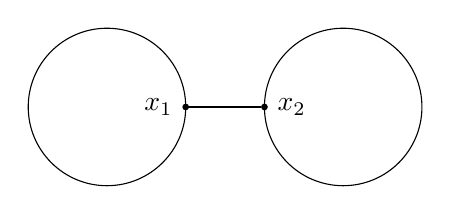
\begin{tikzpicture}
 \tikzset{point/.style = {draw, circle, fill=black, minimum size=2pt,inner sep=0pt}}
 \tikzset{->-/.style={decoration={markings,mark=at position #1 with {\arrow{>}}},postaction={decorate}}}
 \def\rad{1cm}
 \def\len{3cm}
 
 \node (C1) at (0,0) {};
 \node (C2) at (\len,0) {};
 \draw (C1) circle (\rad);
 \draw (C2) circle (\rad);
 
 \path (C1) node[point,label={180:$x_1$}] (x1)  at +(0:\rad) {};
 \path (C2) node[point,label={0:$x_2$}] (x2)  at +(180:\rad) {};
 
 \draw (x1) -- (x2);
  
\end{tikzpicture}

\caption{$K_1$}
\end{subfigure}
\begin{subfigure}{0.45\textwidth}
\centering
%auto-ignore
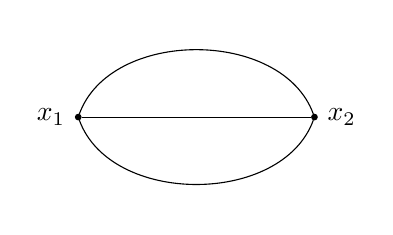
\begin{tikzpicture}
\tikzset{point/.style = {draw, circle, fill=black, minimum size=2pt,inner sep=0pt}}
\node[point,label={180:$x_1$}] (x1) at (0,0) {};
\node[point,label={0:$x_2$}] (x2) at (3,0) {};
\draw[bend left=70] (x1) to (x2);
\draw[bend right=70] (x1) to (x2);
\draw (x1) -- (x2);
\end{tikzpicture}
\caption{$K_2$}
\end{subfigure}
\begin{subfigure}{0.45\textwidth}
\centering
%auto-ignore
\begin{tikzpicture}
 \tikzset{point/.style = {draw, circle, fill=black, minimum size=2pt,inner sep=0pt}}
 \tikzset{->-/.style={decoration={markings,mark=at position #1 with {\arrow{>}}},postaction={decorate}}}
 
 \def\lenI{2.5cm}
 \def\lenII{1cm}
 \def\lenext{0.6cm}
 
 \coordinate[point,label={180:$x_1$}] (x1) at (0,0) {};
 \coordinate[point,label={0:$x_2$}] (x2) at (\lenI,0);
 \path (x1) coordinate[point,label={0:$x_3$}] (x3) at +(60:\lenI);
 
 \draw (x1) -- (x2);
 \draw (x2) -- (x3);
 \draw (x3) -- (x1);
 
 
 \draw (x3) -- +(90:\lenext) node[point,style={fill=white},label={180:$\NVol$}] {};
 \draw (x1) -- +(35:\lenext) node[point,style={fill=white},label={35:$\NOne$}] {};
 \draw (x2) -- +(145:\lenext) node[point,style={fill=white},label={145:$\NOne$}] {};
 
 
\end{tikzpicture}
\caption{Tadpole}
\end{subfigure}
\caption[Graphs $K_1$, $K_2$ and the tadpole graph from Chern-Simons theory.]{Graphs $K_1$ and $K_2$ from the Chern-Simons theory and the tadpole graph with $(l,g)=(2,0)$ for $n=3$.}\label{Fig:K1K2}
\end{figure}
\endgroup }

For $\Sph{3}$, we consider the non-reduced graphs $K_1$ and $K_2$ and the tadpole graph from Figure~\ref{Fig:K1K2}. The graphs $K_1$ and $K_2$ appear in the definition of the Chern-Simons topological invariant in~\cite{Kohno2002} (with a gauge group). The corresponding integrals from our theory vanish ``algebraically'', i.e., at the level of wedge products of $\omega_i$. Indeed, every summand in $K_1$ contains 
\[ \omega_a(x_1,x_1) = 0\quad \text{for some }a=0, 1, 2, \]
and, for degree reasons, the form part of $K_2$ can contain   only
\[ \omega_1(x_1,x_2)^3=0\quad\text{or}\quad\omega_0(x_1,x_2)\omega_{1}(x_1,x_2)\omega_{2}(x_1,x_2)=0.\] 
The tadpole graph contains only
\begin{equation*}
 \omega_2(x_1,x_3)\omega_1(x_1,x_2)\omega_2(x_2,x_3) = 0.\qedhere \end{equation*}
%These relations were checked by the computer. 
%The precise relation to the integrals from perturbative Chern-Simons theory is one of our research goals and may be discussed more in~\cite{MyPhD}.
\qedhere
%It was checked numerically that there are graphs with $C=4$ which do not vanish algebraically.
\end{Remark}

Equations in Remark~\ref{Rem:GraphsThreeSphere} were checked by the computer---this is possible as the vanishing is purely algebraic.
Any author's attempts to show numerically that some integrals are non-zero or get a hint for ``analytic vanishing'' failed so far.
The program for Wolfram Mathematica~10.4 will be made available at \cite{sourcecode} and possibly updated. 


We will now compute $\PMC_{20}$ for $\Sph{1}$, which according to Proposition~\ref{Prop:TotalVanishing} consists only of contributions from the $O_k$-graphs with $k$ even. 
%$L_1, L_3^b$ such that the first boundary component has valency $a$.
By analogy with the finite dimensional case (see~Appendix~\ref{Section:Appendix}), we expect that the number $(-1)^{\sigma_L}I(\sigma_L)$ does not depend on $L$. All inputs are namely the same and the degrees even, i.e., $|m_2^+| = -2$, $|\SuspU^2\Prpg| = -2$ and $|\NVol| = 0$. 

We fix $s_1$, $s_2\ge 1$ such that $k=s_1+s_2$ is even and make the ansatz
\begin{equation*}
n_{20}(\Susp \NVol^{s_1}\otimes  \Susp \NVol^{s_2}) \coloneqq \varepsilon(s_1,s_2) C(s_1,s_2) I(k),
\end{equation*}
where $I(k)$ is the integral
\begin{equation} \label{Eq:Ik}
\frac{1}{V^k}\int_{x_1, \dotsc, x_{k}} G(x_1,x_2) \dotsm G(x_{k-1},x_{k})G(x_{k},x_1)\Vol(x_1) \dotsm \Vol(x_{k}), \end{equation}
$\varepsilon(s_1,s_2)$ a sign and $C(s_1,s_2)$ a combinatorial coefficient to be determined.

We fix a circle in the plane with $k$ points (=\,internal vertices) and denote by $O(s_1,s_2)$ the set of ribbon graphs constructed by attaching external legs from which $s_1$ points in the interior and $s_2$ in the exterior, or the other way round, so that $O(s_1,s_2) = O(s_2, s_1)$ (see Figure~\ref{Fig:Gamma0}). Recall that the ribbon structure is induced from the counterclockwise orientation of the plane. It is easy to see that all graphs in $O(s_1,s_2)$ admit a labeling which is admissible with respect to $\Susp \NVol^{s_1} \otimes \Susp \NVol^{s_2}$, and that $O(s_1,s_2)$ contains a representative of every such $O_k$-graph. 

\Correct[inline,caption={DONE Sign not necessary}]{There is no need to write $(-1)^{k+1}$ when we know that $k$ is even!!! Who cares? Let's keep it so that it is clear where the sign comes from.}
\begin{Lemma}[Integral for the $O_k$-graph for $\Sph{1}$] \label{Lemma:IntegralFor1}
For every even $k\ge 2$, the integral $I(k)$ is equal to
 \begin{equation}\label{Eq:TheFormulaForIk}
 (-1)^{k+1} \frac{1}{2^k}\sum_{i=2, 4, \dotsc ,k} \frac{i}{(i+1)!} \sum_{\substack{i_1+ \dotsb +i_r = k-i \\ i_1, \dotsc, i_r \in 2\N,\, r\in \N}} (-1)^r \frac{1}{(i_1+1)! \dotsm (i_r+1)!}.
 \end{equation}
\end{Lemma}

\begin{proof}
Denote $\bar{\Prpg} \coloneqq -2\pi \Prpg$. For all $k$, $l \ge 1$, we consider the more general integral
\[ I(k,l) \coloneqq \int_{x_1, \dotsc, x_k} \bar{\Prpg}(x_1,x_2) \dotsm \bar{\Prpg}(x_{k-1},x_k) \bar{\Prpg}(x_k,x_1)^l\Vol(x_1) \dotsm \Vol(x_k). \]
Taking the pullback along $(x_1, x_2, \dotsc, x_{k-1}, x_k) \mapsto (x_k, x_{k-1}, \dotsc, x_2, x_1)$ and using the antisymmetry of $\bar{\Prpg}(x,y)$, we get $I(k,l) = 0$ whenever $k+l$ is even. We will compute $I(k,1)$ for $k\in 2\N$ from a recursive relation which arises from successive integration.

For the recursion step, we need to evaluate the integral 
\[\int_{y} \bar{\Prpg}(x,y)\bar{\Prpg}(y,z)^l \Vol(y)\]
for fixed $(x,z)\in (\Sph{1}\times \Sph{1})\backslash\Diag$. Pick the chart $g: \Sph{1}\backslash\{z\} \rightarrow (-\pi,\pi)$ defined by 
\[ g(y)= \bar{\Prpg}(y,z) =  \pi - \alpha(y,z) \quad\text{for } y\in \Sph{1}\backslash\{z\}, \]
where the angle $\alpha$ was defined in Example~\ref{Example:Circle}. It holds $\Diff{g}(y) = \Vol(y)$ and
\[ \bar{\Prpg}(x,y) = \begin{cases} \bar{\Prpg}(x,z) - g(y) - \pi & \text{for }-\pi< g(y)< \bar{\Prpg}(x,z), \\
\bar{\Prpg}(x,z) - g(y) + \pi & \text{for }\bar{\Prpg}(x,z)<g(y)<\pi.
 \end{cases}\]
We compute
\begin{align*}
\int_{y} \bar{\Prpg}(x,y)\bar{\Prpg}(y,z)^l \Vol(y) &= \begin{multlined}[t] \int_{-\pi}^{\pi} (\bar{\Prpg}(x,z) - g)g^l \Diff{g} - \pi \int_{-\pi}^{\bar{\Prpg}(x,z)} g^l \Diff{g} \\ {}+ \pi \int_{\bar{\Prpg}(x,z)}^\pi g^l \Diff{g} \end{multlined} \\
 &=  \frac{2\pi}{l+1} \begin{cases}
  \pi^l \bar{\Prpg}(x,z) - \bar{\Prpg}(x,z)^{l+1} & \text{for }l\text{ even},\\[2ex]
  \dfrac{\pi^{l+1}}{l+2} - \bar{\Prpg}(x,z)^{l+1} & \text{for }l \text{ odd}.
 \end{cases}
\end{align*}


From now on, $\int$ will stand for the Riemannian integral, i.e., $\int f \coloneqq \int f\Vol$ for a function~$f$. We compute
%
\begin{align*}
I(2,l) &= \int_{x_1, x_2} \bar{\Prpg}(x_1,x_2)\bar{\Prpg}(x_2,x_1)^{l} \\
 &= - \int_{y z} \bar{\Prpg}(y,z)^{l+1} \\
 &=- 2\pi \int_{-\pi}^\pi g^{l+1} \Diff{g} \\
 &= \begin{cases} 0 & \text{for }l \text{ even}, \\[2ex] 
 - \dfrac{4 \pi^{l+3}}{l+2} &\text{for }l\text{ odd}. \end{cases}
\end{align*}
For $k\ge 4$ even and $l$ odd, we compute % 10.10.17
\begin{align*}
 I(k,l) &= \begin{multlined}[t]\frac{2\pi}{l+1}\int_{x_1, \dotsc, x_{k-1}}\bar{\Prpg}(x_1,x_2)\dotsm \bar{\Prpg}(x_{k-2},x_{k-1}) \\ \Bigl(\frac{\pi^{l+1}}{l+2} - \bar{\Prpg}(x_{k-1},x_1)^{l+1}\Bigr) \end{multlined} \\ 
&\begin{multlined}
=\frac{-4\pi^2}{(l+1)(l+2)} \int_{x_1, \dotsc, x_{k-2}}\ \bar{\Prpg}(x_1,x_2) \dotsm \bar{\Prpg}(x_{k-3},x_{k-2})\\ \Bigl(\pi^{l+1} \bar{\Prpg}(x_{k-2},x_1)
 -\bar{\Prpg}(x_{k-2},x_1)^{l+2}\Bigr)
\end{multlined} \\
&= \frac{4\pi^2}{(l+1)(l+2)}\bigl(-\pi^{l+1} I(k-2,1)+I(k-2,l+2)\bigr).
\end{align*}
%
%where we used that $\int_{x_{k-1}} \bar{\Prpg}(x_{k-2},x_{k-1}) = 0$.
For the second equality, we used $\int_{x_1} \bar{\Prpg}(x_1,x_2) = 0$ to show that the term multiplied by $\frac{\pi^{l+1}}{l+2}$ vanishes. It follows that
%\[ I_{n,1} = -\frac{(2\pi^2)^n}{(n+1)(n-1)!}-\sum_{l=2,4,\ldots,n-2} \frac{(2\pi^2)^{n-l}}{(n-l+1)!} I_{l,1}\qquad\text{for all }n=2,4,\ldots\]
\begin{align*}
I(k,1) &= \frac{(2\pi)^{k-2}}{(k-1)!} I(2,k-1) - \sum_{l=2, 4, \dotsc, k-2} \frac{(2\pi^2)^{k-l}}{(k-l+1)!} I(l,1) \\ 
&=-\frac{k(2\pi^2)^k}{(k+1)!}-\sum_{l=2, 4, \dotsc, k-2} \frac{(2\pi^2)^{k-l}}{(k-l+1)!} I(l,1)\qquad\text{for all }k=2,\,4,\,\dotsc
\end{align*}
This is a recursive equation of the form $a_k = c_k + \sum_{l=1}^{k-1} d_{k-l} a_l$. Its solution is $a_k = \sum_{i=1}^k c_i D_{k-i}$ with $D_0\coloneqq 1$ and $D_i = \sum d_{i_1} \dotsm d_{i_r}$, where we sum over all $r=1$,~$\dotsc$, $i$ and $i_1$,~$\dotsc$, $i_r\in \N$ such that $i_1+ \dotsb + i_r = i$. Therefore, we get % Proved on 11.10.17, checked by Mathematica in CircularIntCircle.nb
\[ I(k,1) = -(2\pi^2)^k \sum_{i=2, 4, \dotsc, k} \frac{i}{(i+1)!} \sum_{\substack{i_1 + \dotsb + i_r = k-i \\ i_1, \dotsc, i_r \in 2\N, r\in \N}} (-1)^r \frac{1}{(i_1+1)! \dotsm (i_r+1)!}.\]
The result has to be multiplied by $(-1)^k(2\pi)^{-2k}$ in order to get $I(k)$. 
\end{proof} % Checked on 24.3.18.


%\begin{figure}
%\begin{center}
%\includegraphics[width=0.5\textwidth, trim=0.1cm 26cm 15cm 0.1cm,clip]{\GraphicsFolder/circle_xab.pdf}
%\end{center}
%\caption{dasda}
%\end{figure}

\begin{Lemma}[Independence of labeling]\label{Lemma:Independence}
The summand $(-1)^{\sigma_L} I(\sigma_L)$ in the definition of $\PMC_{20}(\Susp\NVol^{s_1}\otimes \Susp\NVol^{s_2})$ for $\Sph{1}$ is independent of the choice of $\Gamma\in O(s_1,s_2)$ and its labeling $L$ which is compatible and admissible with respect to the input.
\end{Lemma}
\begin{proof}
Pick $\Gamma\in O(s_1,s_2)$ and its admissible labeling $L$. Let $L'$ be an other admissible labeling of $\Gamma$. We distinguish the following situations:
\begin{itemize}
 \item Suppose that $L$ and $L'$ differ by a permutation $\mu$ in $L_3^b$. A similar argument as in the proof of Lemma~\ref{Lem:MCCond} shows that $(-1)^{\sigma_{L'}} = (-1)^\mu (-1)^{\sigma_L}$ and $I(\sigma_L') = (-1)^\mu I(\sigma_L)$, where the sign in the integral comes from the permutation of $\Vol$'s, which have form-degree $1$. Hence $(-1)^{\sigma_{L'}}I(\sigma_{L'}) = (-1)^{\sigma_{L}}I(\sigma_{L})$.
\item Suppose that the boundaries are permuted, i.e., that~$L$ and~$L'$ differ in~$L_1^b$. Notice that~$s_1=s_2$ because otherwise one of~$L$ or~$L'$ would not be admissible. The sign from changing~$L_1^b$ cancels as in the previous case. 
%In order to preserve compatibility with $L_1$ we must have $L_2' \neq L_2$. But this was handled in the previous case.
\item Suppose that $L$ and $L'$ differ in $L_2$. It was explained in the proof of Lemma~\ref{Lem:MCCond} that a single change of $L_2$ induces the sign $(-1)^{n-1} = 1$ in $(-1)^{\sigma_L} I(\sigma_L)$.  
\item A cyclic permutation in $L_3^v$ induces a sign neither in $(-1)^{\sigma_L}$ nor in $I(\sigma_L)$.
 \item A permutation $\mu$ in $L_1^v$ induces $(-1)^\mu$ in $(-1)^{\sigma_L}$ and a change in $I(\sigma_L)$, which can be realized by taking the pullback along $\mu: (x_1,\ldots,x_k)\mapsto (x_{\mu_1},\ldots,x_{\mu_k})$. However, the sign of the Jacobian is $(-1)^\mu$, which cancels the sign from $(-1)^{\sigma_L}$.
\end{itemize}

\begin{figure}[t]
\centering
%auto-ignore
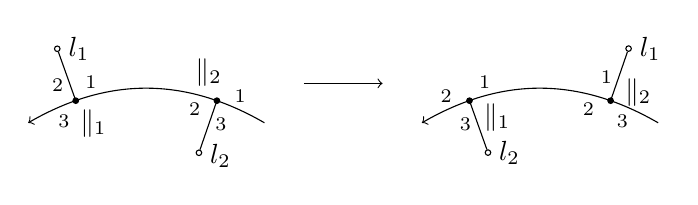
\begin{tikzpicture}

\def\rad{10cm}
\def\angdist{30}
\def\posa{75}
\def\extlen{0.7cm}
\def\delta{5}
\def\startpos{0.2}
\def\endpos{0.8}
\def\labeldelta{0.003}
\def\labelrad{0.15}

\tikzset{point/.style = {draw, circle, fill=black, minimum size=2pt, inner sep=0pt}}
\tikzset{->-/.style={decoration={markings,mark=at position #1 with {\arrow{>}}},postaction={decorate}}}
\tikzset{-<-/.style={decoration={markings,mark=at position #1 with {\arrow{<}}},postaction={decorate}}}
% C1

\draw [<-] (0,0) to[bend left] coordinate [pos=\startpos-\labeldelta] coordinate [pos=\startpos-0.01, below] (v11d) coordinate [pos=\startpos, below] (v11) coordinate [pos=\startpos+\labeldelta] coordinate [pos=\endpos-0.01, below] (v12d) coordinate [pos=\endpos, below] (v12) (3,0);

\node[point] at (v11) {};
\node[point] at (v12) {};

\path (v11) node at +(50:2*\labelrad){\scriptsize{1}};
\path (v11) node at +(140:2*\labelrad){\scriptsize{2}};
\path (v11) node at +(240:2*\labelrad){\scriptsize{3}};

\path (v12) node at +(10:2*\labelrad){\scriptsize{1}};
\path (v12) node at +(200:2*\labelrad){\scriptsize{2}};
\path (v12) node at +(280:2*\labelrad){\scriptsize{3}};

\draw [<-] (5,0) to[bend left] coordinate [pos=\startpos-0.01, below] (v21d) coordinate [pos=\startpos, below] (v21) coordinate [pos=\endpos-0.01, below] (v22d) coordinate [pos=\endpos, below] (v22) (8,0);
\draw [-{>[scale=1.5]}] (3.5,0.5) -- (4.5,0.5);

\node[point] at (v21) {};
\node[point] at (v22) {};

\path (v11d) -- (v11) -- ([turn]90:\extlen) coordinate[point,style={fill=white}] (v11l);
\path (v12d) -- (v12) -- ([turn]-90:\extlen) coordinate[point,style={fill=white}] (v12l);

\draw (v11) node [inner sep=0pt,label={[yshift=1pt,xshift=-2pt]-80:$\Vert_1$}] {}  node [inner sep=0pt] {} -- (v11l) node [label={[xshift=-3pt]0:$l_1$}] {};
\draw (v12) node [inner sep=0pt,label={[xshift=-3pt,yshift=1pt]90:$\Vert_2$}] {} node [inner sep=0pt] {} node [inner sep=0pt] {} node [inner sep=0pt] {} -- (v12l)  node [label={[xshift=-3pt,yshift=-1pt]0:$l_2$}] {};

\path (v21d) -- (v21) -- ([turn]-90:\extlen) coordinate[point,style={fill=white}] (v21l);
\path (v22d) -- (v22) -- ([turn]90:\extlen) coordinate[point,style={fill=white}] (v22l);


\path (v21) node at +(50:2*\labelrad){\scriptsize{1}};
\path (v21) node at +(170:2*\labelrad){\scriptsize{2}};
\path (v21) node at +(260:2*\labelrad){\scriptsize{3}};

\path (v22) node at +(100:2*\labelrad){\scriptsize{1}};
\path (v22) node at +(200:2*\labelrad){\scriptsize{2}};
\path (v22) node at +(300:2*\labelrad){\scriptsize{3}};

\draw (v21) node [inner sep=0pt,label={[yshift=-6pt,xshift=1pt]0:$\Vert_1$}] {} node [inner sep=0pt] {}  node [inner sep=0pt] {}  node [inner sep=0pt] {} -- (v21l) node [label={[xshift=-3pt]0:$l_2$}] {};


\draw (v22) node [inner sep=0pt,label={[yshift=3pt,xshift=1pt]0:$\Vert_2$}] {} node [inner sep=0pt] {}  node [inner sep=0pt] {}  node [inner sep=0pt] {} -- (v22l) node [label={[xshift=-3pt]0:$l_1$}] {};;


\end{tikzpicture}
\caption[Swap of adjacent vertices on a circular graph.]{Swapping adjacent legs.}\label{Fig:TwoLegs}
\end{figure}

Next, we prove the independence of $\Gamma\in O(s_1,s_2)$. Let $L$ be an admissible and compatible labeling of $\Gamma$. Pick two adjacent internal vertices with external legs pointing to different regions, i.e., one to the interior of the circle and the other to the exterior. Suppose that the vertices are labeled by $\Vert_1$ and $\Vert_2$ and the legs by $l_1$ and $l_2$, respectively. Let $\Gamma'\in O(s_1,s_2)$ be the graph with the two legs turned inside out (see Figure~\ref{Fig:TwoLegs}). We can construct an admissible and compatible labeling $L'$ of $\Gamma'$ by making the following changes to $L$: The new leg at $\Vert_1$ will be labeled by $l_2$ and the new leg at $\Vert_2$ by $l_1$.
%This produces $-1$ in $(-1)^{\sigma_L - \sigma_{L'}}$.
The cyclic orderings at $\Vert_1$ and $\Vert_2$, respectively, have to be modified by a transposition in order to get compatibility with the new ribbon structure. All other labelings can be copied from $L$.
%This does not produce a sign as the change is in pair.
In total, we get
\[ (-1)^{\sigma_L - \sigma_{L'}} = -1. \]
This sign is compensated by swapping the one-forms in $I(\sigma_L)$:
\[ \Vol (x_{\Vert_1}) \dots \Vol(x_{\Vert_2}) \;\longleftrightarrow\;\Vol(x_{\Vert_2}) \dots \Vol(x_{\Vert_1}). \]
The independence of $\Gamma\in O(s_1,s_2)$ follows from the fact that we can span the entire $O(s_1,s_2)$ by repeating the swap-of-legs operation.
\end{proof}

\begin{Lemma}[Sign]\label{Lemma:SignForMCOnCircle}
We have
\[\varepsilon(s_1,s_2) = (-1)^{s_1+1}. \]
\end{Lemma}
\begin{proof} 

\begin{figure}
\centering
%auto-ignore
\begin{tikzpicture}

\def\rad{3cm}
\def\angdist{40}
\def\posa{90}
\def\posb{270}
\def\delta{15}
\def\orientrad{0.5cm}
\def\orientang{270}
\def\extlen{1.2cm}
\def\halflabeldelta{5}
\def\halflabeldeltarad{0.15cm}
\def\verthalflabeldeltarad{0.45cm}
\def\verthalflabeldelta{3}

\tikzset{point/.style = {draw, circle, fill=black, minimum size=2pt,inner sep=0pt}}
\tikzset{->-/.style={decoration={markings,mark=at position #1 with {\arrow{>}}},postaction={decorate}}}


% Boundary labels
\node (C) at (2,1) {1};
\node (D) at (6,3.5) {2};

% Edges
\draw[->-=0.5] ([shift=(\posa-2*\angdist:\rad)]C) arc (\posa-2*\angdist:\posa-\angdist:\rad) node[midway,right=2pt,yshift=2pt]{$\GKer_{1}$};
\draw[->-=0.5] ([shift=(\posa-\angdist:\rad)]C) arc (\posa-\angdist:\posa:\rad) node[midway,above,xshift=3pt]{$\GKer_k$};
\draw[->-=0.5] ([shift=(\posa:\rad)]C) arc (\posa:\posa+\angdist:\rad) node[midway,above=2pt,xshift=-3pt]{$\GKer_{k-1}$};
\draw[->-=0.5] ([shift=(\posb:\rad)]C) arc (\posb:\posb+\angdist:\rad) node[midway,below=3pt,xshift=8pt]{$\GKer_{k-s_1}$};

%Additional delta to edges
\draw([shift=(\posb-\delta:\rad)]C) arc (\posb-\delta:\posb:\rad);
\draw([shift=(\posb+\angdist:\rad)]C) arc (\posb+\angdist:\posb+\angdist+\delta:\rad);
\draw([shift=(\posa+\angdist:\rad)]C) arc (\posa+\angdist:\posa+\angdist+\delta:\rad);
\draw([shift=(\posa-2*\angdist-\delta:\rad)]C) arc (\posa-2*\angdist-\delta:\posa-2*\angdist:\rad);

%Boundary orientation
\draw[->] ([shift=(\orientang:\orientrad)]C) arc (\orientang:0:\orientrad);
\draw[->] ([shift=(0:\orientrad)]D) arc (0:\orientang:\orientrad);

% Dashed lines
\draw[dashed]([shift=(\posa+\angdist+\delta:\rad)]C) arc (\posa+\angdist+\delta:\posb-\delta:\rad);
\draw[dashed]([shift=(\posb+\angdist+\delta:\rad)]C) arc (\posb+\angdist+\delta:360+\posa-2*\angdist-\delta:\rad);

% Internal vertices
\path (C) node[point,label={90:$x_1$}] (x1)  at +(\posa:\rad){};
\path (C) node[point,label={[label distance=-3pt]160:$x_2$}] (x2)  at +(\posa+\angdist:\rad){};
\path (C) node[point,label={[label distance=]0:$x_k$}] (xk)  at +(\posa-\angdist:\rad){};
\path (C) node[point,label={[label distance=-1pt]-15:$x_{k-1}$}] (xkk) at +(\posa-2*\angdist:\rad){};

\path (C) node[point,label={[label distance=]-90:$x_{s_1}$}] (xa) at +(\posb:\rad){};
\path (C) node[point,label={[label distance=2pt]360:$x_{s_1+1}$}] (xaa) at +(\posb+\angdist:\rad){};

% External legs
\path (C) -- (x1) -- ([turn]180:\extlen) coordinate (vx1) {};
\path (C) -- (x2) -- ([turn]180:\extlen) coordinate (vx2) {};
\path (C) -- (xk) -- ([turn]0:\extlen) coordinate (vxk) {};
\path (C) -- (xkk) -- ([turn]0:\extlen) coordinate (vxkk) {};
\path (C) -- (xa) -- ([turn]180:\extlen) coordinate (vxa) {};
\path (C) -- (xaa) -- ([turn]0:\extlen) coordinate (vxaa) {};

\path[draw] (x1)--(vx1);


\draw (x1) -- (vx1) node[point,style={fill=white},label={0:$\NVol_{s_1}$}] {};
\draw (x2) -- (vx2) node[point,style={fill=white},label={0:$\NVol_{s_1-1}$}] {};
\draw (xk) -- (vxk) node[point,style={fill=white},label={0:$\NVol_{k}$}] {};
\draw (xkk) -- (vxkk) node[point,style={fill=white},label={0:$\NVol_{k-1}$}] {};
\draw (xa) -- (vxa) node[point,style={fill=white},label={0:$\NVol_{1}$}] {};
\draw (xaa) -- (vxaa) node[point,style={fill=white},label={0:$\NVol_{s_1+1}$}] {};

% Halfedge labeling 

\path (C) +(\posa+\halflabeldelta:\rad-\halflabeldeltarad) node {{\scriptsize 2}};
\path (C) +(\posa-\halflabeldelta:\rad-\halflabeldeltarad) node {{\scriptsize 1}};
\path (C) +(\posa+\angdist+\halflabeldelta:\rad-\halflabeldeltarad) node {{\scriptsize 2}};
\path (C) +(\posa+\angdist-\halflabeldelta:\rad-\halflabeldeltarad) node {{\scriptsize 1}};
\path (C) +(\posa-\angdist+\halflabeldelta:\rad-\halflabeldeltarad) node {{\scriptsize 3}};
\path (C) +(\posa-\angdist-\halflabeldelta:\rad-\halflabeldeltarad) node {{\scriptsize 1}};
\path (C) +(\posa-2*\angdist+\halflabeldelta:\rad-\halflabeldeltarad) node {{\scriptsize 3}};
\path (C) +(\posa-2*\angdist-\halflabeldelta:\rad-\halflabeldeltarad) node {{\scriptsize 1}};
\path (C) +(\posb+\halflabeldelta:\rad-\halflabeldeltarad) node {{\scriptsize 2}};
\path (C) +(\posb-\halflabeldelta:\rad-\halflabeldeltarad) node {{\scriptsize 1}};
\path (C) +(\posb+\angdist+\halflabeldelta:\rad-\halflabeldeltarad) node {{\scriptsize 3}};
\path (C) +(\posb+\angdist-\halflabeldelta:\rad-\halflabeldeltarad) node {{\scriptsize 1}};

\path (C) +(\posa-\verthalflabeldelta:\rad-\verthalflabeldeltarad) node {{\scriptsize 3}};
\path (C) +(\posa+\angdist-\verthalflabeldelta:\rad-\verthalflabeldeltarad) node {{\scriptsize 3}};
\path (C) +(\posa-\angdist+\verthalflabeldelta:\rad+.7*\verthalflabeldeltarad) node {{\scriptsize 2}};
\path (C) +(\posa-2*\angdist+\verthalflabeldelta:\rad+.7*\verthalflabeldeltarad) node {{\scriptsize 2}};

\path (C) +(\posb+\angdist-\verthalflabeldelta:\rad+.7*\verthalflabeldeltarad) node {{\scriptsize 2}};
\path (C) +(\posb-\verthalflabeldelta:\rad-\verthalflabeldeltarad) node {{\scriptsize 3}};
\end{tikzpicture}
%\includegraphics[width=0.6\textwidth, trim=5.6cm 20.6cm 5.3cm 1.2cm,clip]{\GraphicsFolder/reference_labeling_of_circle.pdf}
\caption[A fully labeled circular ribbon graph for $\Sph{1}$.]{The graph $\Gamma^*$ with the labeling $L^*$. It can be checked that~$L_1$ and~$L_2$ are compatible.}\label{Fig:Gamma0}
\end{figure}


By Lemma~\ref{Lemma:Independence}, in order to compute $(-1)^{\sigma_L}I(\sigma_L)$, we can pick $\Gamma^*\in O(s_1,s_2)$ and its admissible and compatible labeling $L^*$ from Figure~\ref{Fig:Gamma0}. We abbreviate $\sigma_0 = \sigma_{L^*}$. The corresponding integral \eqref{Eq:ISigma} reads
\[ I(\sigma_0) = \begin{multlined}[t] \frac{1}{V^k}\int_{x_1, \dotsc, x_k} G(x_{k-1},x_k) \dotsm G(x_{1},x_2)G(x_k,x_1) \Vol(x_{s_1}) \dotsm \Vol(x_1)\\ \Vol(x_{s_1+1}) \dotsm \Vol(x_k). \end{multlined} \]
It differs from $I(k)$ from~\eqref{Eq:Ik} in the order of $\Prpg$'s and $\Vol$'s. A reordering produces the sign
\[(-1)^{\frac{1}{2}s_1(s_1-1)}.\] 
We will compute $(-1)^{\sigma_0}$ by ordering half-edges from the edge order back to the vertex order while looking at Figure~\ref{Fig:Gamma0}. The steps are as follows: 
\begin{itemize}
 \item Transpose half-edges at internal vertices so that the first half-edge goes inside the vertex and the third outside with respect to the counterclockwise orientation. This gives $(-1)^a$.
 \item Permute external legs so that $\NVol_i$ is at $x_i$ for all $i=1$, $\dotsc$, $k$. This gives 
 \[(-1)^{\frac{1}{2}s_1(s_1-1)}. \]
 \item Permute internal edges so that $\Prpg_i$ starts at the third half-edge of $x_i$ and ends at the first half-edge of $x_{i+1}$ for all $i=1$, $\dotsc$, $k-1$. This does not produce any sign as swapping of two $\Prpg$'s requires two transpositions.
 \item  At this point, we have the permutation
 \[\begingroup\setlength\arraycolsep{4pt}      \begin{pmatrix}
 1 & 2 &\dots & 2(e-1)-1 & 2(e-1) & 2e-1 & 2e & 2e + 1 & \dots & 3k \\
 3 & 4 &\dots & 3k-3 & 3k-2 &  3k &  1 & 2 & \dots & 3k-1
 \end{pmatrix}.\endgroup\]
We interpret the last line as $\Prpg_1\dots \Prpg_k \NVol_1\dots \NVol_k$ and permute it to the sequence $\NVol_1 \Prpg_1 \NVol_2 \Prpg_2\dots \NVol_k \Prpg_k$, which does not produce any sign. We end up with 
\[ \sigma_0' = \begin{pmatrix}
 1 & 2 & 3 & \dots & 3k-1 & 3k \\
 2 & 3 & 4 & \dots & 3k & 1
\end{pmatrix}. \]
It is now easy to see that
\[ (-1)^{\sigma_0'} = (-1)^{3k-1}. \]
\end{itemize}
In total, we get
\[ (-1)^{\sigma_0} = (-1)^{s_1 + \frac{1}{2}s_1(s_1-1) + k + 1}. \]
As for the other signs in Definition~\ref{Def:PushforwardMCdeRham}, we have $s(k,l) = k + \frac{1}{2}k(k-1)$ and $P(\NVol^k) = \frac{1}{2}k(k-1)$. There is no sign from $\Susp^2 \NVol^{s_1}\otimes \NVol^{s_2} = \Susp \NVol^{s_1} \otimes \Susp \NVol^{s_2}$ since $\Abs{\Susp} = -2$. Multiplying everything together, we get $\varepsilon(s_1,s_2)$.
\end{proof}
\begin{figure}
\centering
%auto-ignore
\begin{tikzpicture}

\def\rad{1cm}
\def\angdist{60}
\def\posa{90}
\def\extlen{0.5cm}
\def\delta{20}

\tikzset{point/.style = {draw, circle, fill=black, minimum size=2pt,inner sep=0pt}}
\tikzset{->-/.style={decoration={markings,mark=at position #1 with {\arrow{>}}},postaction={decorate}}}
\tikzset{-<-/.style={decoration={markings,mark=at position #1 with {\arrow{<}}},postaction={decorate}}}
% C1

\coordinate (C1) at (0,0) {};
\coordinate (C2) at (4*\rad,0) {};
\coordinate (C3) at (8*\rad,0) {};

\path (C1) node[point,label={270:1}] (C11)  at +(\posa:\rad) {};
\path (C1) node[point,label={[label distance=-3pt]30:2}] (C12)  at +(\posa-\angdist:\rad) {};
\path (C1) node[point,label={[label distance=-3pt]290:k}] (C1k)  at +(\posa+\angdist:\rad) {};

\draw ([shift=(\posa:\rad)]C1) arc (\posa:\posa+\angdist:\rad);
\draw[-<-=0.5] ([shift=(\posa-\angdist:\rad)]C1) arc (\posa-\angdist:\posa:\rad);

\draw ([shift=(\posa+\angdist:\rad)]C1) arc (\posa+\angdist:\posa+\angdist+\delta:\rad);
\draw ([shift=(\posa-\angdist-\delta:\rad)]C1) arc (\posa-\angdist-\delta:\posa-\angdist:\rad);

\draw[dashed]([shift=(\posa+\angdist+\delta:\rad)]C1) arc (\posa+\angdist+\delta:360+\posa-\angdist-\delta:\rad);



% C2

\path (C2) node[point,label={[label distance=-1pt]90:$\bar{1}$}] (C21)  at +(\posa:\rad) {};
\path (C2) node[point,label={[label distance=-3pt]30:$\bar{k}$}] (C2k)  at +(\posa-\angdist:\rad) {};
\path (C2) node[point,label={[label distance=-3pt]290:$\bar{2}$}] (C22)  at +(\posa+\angdist:\rad) {};

\draw[->-=0.5]  ([shift=(\posa:\rad)]C2) arc (\posa:\posa+\angdist:\rad);
\draw ([shift=(\posa-\angdist:\rad)]C2) arc (\posa-\angdist:\posa:\rad);

\draw ([shift=(\posa+\angdist:\rad)]C2) arc (\posa+\angdist:\posa+\angdist+\delta:\rad);
\draw ([shift=(\posa-\angdist-\delta:\rad)]C2) arc (\posa-\angdist-\delta:\posa-\angdist:\rad);

\draw[dashed]([shift=(\posa+\angdist+\delta:\rad)]C2) arc (\posa+\angdist+\delta:360+\posa-\angdist-\delta:\rad);

% C3

\path (C3) node[point,label={[label distance=0pt]90:$\bar{k}$}] (C3k)  at +(\posa:\rad) {};
\path (C3) node[point,label={[label distance=-3pt]120:$\bar{1}$}] (C31)  at +(\posa+\angdist:\rad) {};
\path (C3) node[point,label={[label distance=-3pt]60:$\bar{2}$}] (C32)  at +(\posa+2*\angdist:\rad) {};

\draw[->-=0.5] ([shift=(\posa+\angdist:\rad)]C3) arc (\posa+\angdist:\posa+2*\angdist:\rad);
\draw ([shift=(\posa:\rad)]C3) arc (\posa:\posa+\angdist:\rad);

\draw ([shift=(\posa+2*\angdist:\rad)]C3) arc (\posa+2*\angdist:\posa+2*\angdist+\delta:\rad);
\draw ([shift=(\posa-\delta:\rad)]C3) arc (\posa-\delta:\posa:\rad);

\draw[dashed]([shift=(\posa+2*\angdist+\delta:\rad)]C3) arc (\posa+2*\angdist+\delta:360+\posa-\delta:\rad);

% Arrows

\draw[-{>[scale=1.0]}] ($(C1)+(1.5*\rad,0)$) -- ($(C1)+(2.5*\rad,0)$) node[midway,above=2pt]{Inv};
\draw[-{>[scale=1.0]}] ($(C2)+(1.5*\rad,0)$) -- ($(C2)+(2.5*\rad,0)$) node[midway,above]{(-1)};

% External legs

\path (C1) -- (C11) -- ([turn]0:\extlen) coordinate (C11x){};
\path[draw] (C11)--(C11x);
\path (C1) -- (C12) -- ([turn]180:\extlen) coordinate (C12x){};
\path[draw] (C12)--(C12x);
\path (C1) -- (C1k) -- ([turn]0:\extlen) coordinate (C1kx){};
\path[draw] (C1k)--(C1kx);

\path (C2) -- (C21) -- ([turn]180:\extlen) coordinate (C21x){};
\path[draw] (C21)--(C21x);
\path (C2) -- (C22) -- ([turn]0:\extlen) coordinate (C22x){};
\path[draw] (C22)--(C22x);
\path (C2) -- (C2k) -- ([turn]180:\extlen) coordinate (C2kx){};
\path[draw] (C2k)--(C2kx);

\path (C3) -- (C31) -- ([turn]180:\extlen) coordinate (C31x){};
\path[draw] (C31)--(C31x);
\path (C3) -- (C32) -- ([turn]0:\extlen) coordinate (C32x){};
\path[draw] (C32)--(C32x);
\path (C3) -- (C3k) -- ([turn]180:\extlen) coordinate (C3kx){};
\path[draw] (C3k)--(C3kx);


\node[point,style={fill=white}] at (C11x) {};
\node[point,style={fill=white}] at (C12x) {};
\node[point,style={fill=white}] at (C1kx) {};

\node[point,style={fill=white}] at (C21x) {};
\node[point,style={fill=white}] at (C22x) {};
\node[point,style={fill=white}] at (C2kx) {};

\node[point,style={fill=white}] at (C31x) {};
\node[point,style={fill=white}] at (C32x) {};
\node[point,style={fill=white}] at (C3kx) {};
\end{tikzpicture}
\caption[The mirror isomorphism for the $O_k$-graph.]{The mirror isomorphism $M: 1 \dots k \mapsto \bar{k} \dots\bar{1}$ is a composition of the inversion and the counterclockwise rotation by one place.}\label{Fig:Mirror}
\end{figure}
\begin{Lemma}[Combinatorial coefficient]
\label{Lemma:CombinatorialCoefficientForMCOnCircle}
It holds \[C(s_1,s_2) = \frac{1}{2} a k! \binom{k-1}{s_1}.\]
\end{Lemma}
\begin{proof}
Every isomorphism of ribbon graphs $\Gamma$ and $\Gamma'$ from $O(s_1,s_2)$ is a composition of the clockwise rotation $(r)$ for $r\in \Z$ and the mirror operation $M$ defined as follows: If $1$,~$\dotsc$, $k$ label internal vertices in the clockwise direction starting from the north-pole, then the result of $M$ is $\bar{k}$,~$\dotsc$, $\bar{1}$, where $\bar{i}$ means that the external leg is reversed (see Figure~\ref{Fig:Mirror}). These operations satisfy
\[ (r+k) = (r),\; (r)(-r)=\Id,\; M^2 = \Id,\; (r)M = M(-r), \]
and hence generate a group $\mathrm{G}$ which is isomorphic to the dihedral group $\Z_k \rtimes \Z_2$. The orbit space $O(s_1,s_2)/\mathrm{G}$ is in $1:1$ correspondence with isomorphism classes of admissible $O_k$-graphs and $\Aut(\Gamma)$ is in $1:1$ correspondence with $\Stab{\Gamma}$. From the orbit-stabilizer formula, we get
\begin{align*}
\sum_{\substack{[\Gamma] \text{ admiss. }\\O_k-\text{graph}}} \frac{1}{\Abs{\Aut(\Gamma)}} &= \sum_{[\Gamma]\in O(s_1,s_2)/\mathrm{G}} \frac{1}{\Abs{\Stab{\Gamma}}} \\
& = \sum_{\Gamma\in O(s_1,s_2)} \frac{1}{\Abs{\Orb{\Gamma}}\Abs{\Stab{\Gamma}}} \\[2ex]
&= \frac{\Abs{O(s_1,s_2)}}{\Abs{\mathrm{G}}}\\[1ex] 
&= \frac{1}{2k}{\binom{k}{s_1}}\times\begin{cases} 1 & \text{for }s_1=s_2, \\ 2 & \text{for }s_1\neq s_2.\end{cases}
\end{align*}
The two cases are compensated in the sum over labelings: For $s_1=s_2$, both labelings $L_1^b$ are admissible, and hence we get the factor $2$.

Next, we multiply by $k! s_1(k-s_1)$, which is the number of $L_1^v$ and $L_3^b$. There is also the factor $\frac{1}{l!} = \frac{1}{2}$. Multiplying everything together, we get $C(s_1,s_2)$.
%In total we get
%\[ \frac{1}{2} a(k-a) k! \frac{1}{k}{{k}\choose{a}} = \frac{1}{2} a k! \binom{k-1}{a}. \]
\end{proof}

Before we summarize the results of our computations (see Proposition~\ref{Proposition:MCSphere} below), we show directly that $\PMC$ is a Maurer-Cartan element; i.e., in this special case, we do not need general results from \cite{Cieliebak2018} at all.

\begin{Lemma}[Maurer-Cartan equation for $\Sph{n}$] \label{Lem:MCEquation}
For $n\ge 1$, consider $\Sph{n}$ with the Hodge Propagator from~\eqref{Eq:GreenKernelMC1}. The collection $(\PMC_{lg})$ satisfies the Maurer-Cartan equation~\eqref{Eq:MaurerCartanEquation} for $\dIBL(\CycC(\Harm(\Sph{n})))$.
\end{Lemma}

\begin{proof}
%The degree and filtration conditions of Definition~\ref{Def:MaurerCartan} are satisfied by a general $\PMC=(\PMC_{lg})$ from Definition~\ref{Def:PushforwardMCdeRham}.
%
% We will now prove that $\PMC$ for $\Sph{n}$ satisfies the Maurer-Cartan equation~\eqref{Eq:MaurerCartanEquation} by 
We will show that for every $l\ge 1$, $g\ge 0$ all summands in the relation corresponding to $(l,g)$ vanish. The summands for $(l,g)= (1,0)$ are $\OPQ_{110}(\PMC_{10})$ and $\frac{1}{2}\OPQ_{210}(\PMC_{10},\PMC_{10})$, and the summand for $(l,g)=(2,0)$ is $\OPQ_{120}(\PMC_{10})$.
The first term vanishes trivially as $\OPQ_{110}=0$, while the other two terms vanish by~\cite[Proposition 12.5]{Cieliebak2015} because $\PMC_{10} = \MC_{10}$
is the canonical Maurer-Cartan element. For $(l,g)\neq (1,0)$, we have the following four situations:
\begin{description}[font=\normalfont\itshape]
\item[$\OPQ_{210}\circ_2 \PMC_{lg}$, $l\ge 2$:] 
%The idea is that $\OPQ_{210}$ from~\eqref{Eq:CanonicaldIBLSn} feeds $\NOne$ into one of its inputs, but all graphs with $\NOne$ at an exterior vertex are $0$ by Proposition~\ref{Prop:TotalVanishing}. The precise argument is as follows. 
Let $\Psi = \Psi_1 \cdots \Psi_l\in \Ext_l \CycC$ be a summand of $\PMC_{lg}$. 
 From Proposition~\ref{Prop:TotalVanishing} it follows that the summands can be chosen such that $\Psi_1$,~$\dotsc$, $\Psi_l \in \DBCycRed\Harm(\Sph{n})[3-n]$, i.e., such that $\Psi_i$ evaluates to $0$ whenever $\NOne$ is a part of its argument. From Definition~\ref{Def:CircS}, we compute
\[\OPQ_{210}\circ_2 (\Psi_1\cdots\Psi_l) = \sum_{\sigma\in \Perm_{2,l-2}} \varepsilon(\sigma,\Psi)\OPQ_{210}(\Psi_{\sigma_1^{-1}}\cdot\Psi_{\sigma_2^{-1}})\cdot\Psi_{\sigma_3^{-1}}\cdots \Psi_{\sigma_l^{-l}}. \]
We clearly have $\OPQ_{210}(\Psi_{\sigma_1^{-1}}\cdot\Psi_{\sigma_2^{-1}})=0$ because $\OPQ_{210}$ feeds $\NOne$ into one of its inputs. It follows that $\OPQ_{210}\circ_2 \PMC_{lg} = 0$.

\item[$\OPQ_{210}\circ_{1,1}(\PMC_{l_1 g_1} \odot \PMC_{l_2 g_2})$, $(l_i,g_i) \neq (1,0)$:] A similar argument as above.
\item[$\OPQ_{120}\circ_1 \PMC_{lg}$, $(l,g)\neq(1,0)$:] A similar argument as above using that $\OPQ_{120}$ also feeds~$\NOne$ into its input. 
%also always feeds $\NOne$ into its input.
\item[$\OPQ_{210}\circ_{1,1} (\PMC_{10}\odot \PMC_{lg})$, $(l,g)\neq (1,0)$:] 
As in the case of $\OPQ_{210}\circ_2 \PMC_{lg}$, suppose that $\Psi_1$,~$\dotsc$, $\Psi_l \in \DBCycRed\Harm(\Sph{n})[3-n]$. Recall that we write $\Omega_i = \Susp \omega_i \in \BCyc \Harm(\Sph{n})[3-n]$ and $\Omega = \Omega_1\otimes \dotsb \otimes \Omega_l$. From Definition~\ref{Def:CircS}, we compute
\begin{align*}
&[\OPQ_{210} \circ_{1,1}(\PMC_{10}\odot \Psi)](\Omega_1 \otimes \dotsb \otimes \Omega_l) 
\\ &\quad = \begin{multlined}[t] \Bigl[ \sum_{i=1}^l (-1)^{\Abs{\Psi_i}(\Abs{\Psi_1} + \dotsb + \Abs{\Psi_{i-1}})} \OPQ_{210}(\PMC_{10}\Psi_i)\Psi_1\cdots \widehat{\Psi_i}\cdots \Psi_l\Bigr]\\ (\Omega_1 \otimes \dotsb \otimes \Omega_l) \end{multlined} \\ 
 &\quad = \begin{multlined}[t] \vphantom{\sum_{i}}\smash{\sum_{\substack{\mu \in \Perm_l \\ i=1, \dotsc, l}}} \frac{1}{l!} (-1)^{\Abs{\Psi_i}(\Abs{\Psi_1} + \dotsb + \Abs{\Psi_{i-1}})} \varepsilon(\mu,\Omega) (\OPQ_{210}(\PMC_{10}\cdot\Psi_i)\otimes \Psi_1\otimes \dotsb \\ \widehat{\Psi_i}\dotsb\otimes \Psi_l)(\Omega_{\mu_1^{-1}} \otimes \dotsb \otimes \Omega_{\mu_l^{-1}}). \end{multlined}
\end{align*}
For every $i=1$, $\dotsc$, $l$, we have
 \begin{align*} 
 & \OPQ_{210}(\PMC_{10}\cdot \Psi_i)(\Omega) = \OPQ_{210}(\PMC_{10}\otimes \Psi_i)(\Omega) \\
 & \qquad = \begin{multlined}[t]- \sum \varepsilon(\omega\mapsto \omega^1 \omega^2)[(-1)^{(n-1)\Abs{\omega^1}} \PMC_{10}(\Susp \NOne \omega^1) \Psi_i(\Susp \NVol \omega^2) \\ {}+ (-1)^{\Abs{\omega^1}} \PMC_{10}(\Susp \NVol \omega^1) \Psi_i(\Susp \NOne \omega^2)] \end{multlined} \\ 
 & \qquad = - \sum \varepsilon(\omega\mapsto \omega^1 \omega^2)(-1)^{(n-1)\Abs{\omega^1}} \PMC_{10}(\Susp \NOne \omega^1) \Psi_i(\Susp \NVol \omega^2).
\end{align*}
This can be non-zero only if $\omega = \NOne \NVol^{s-1}$ for some $s\ge 2$ (up to a cyclic permutation). For this input, we get
\begin{align*} &\OPQ_{210}(\PMC_{10}\cdot \Psi_i)(\Susp \NOne \NVol^{s-1}) \\ &\quad = \begin{aligned}[t]
&-[\varepsilon(\NOne \NVol^{s-1} \mapsto \NOne\NVol^{s-1})\PMC_{10}(\Susp \NOne\NOne\NVol)\Psi_i(\Susp\NVol^{s-1}) \\
&{}+ \varepsilon(\NOne \NVol^{s-1} \mapsto \NVol\NOne\NVol^{s-2})\PMC_{10}(\Susp \NOne\NVol\NOne)  \Psi_i(\Susp\NVol^{s-1})] \end{aligned} \\
 &\quad= (-1)^{n-3}[1+(-1)^{ns+s-1}] \Psi_i(\Susp\NVol^{s-1}).
\end{align*}
The prefactor in brackets is $0$ for $n$ odd or $s$ even, whereas $\NVol^{s-1} = 0$ for $n$ even and~$s$ odd. Therefore,  we have $\OPQ_{210}\circ_{1,1} (\PMC_{10}\odot \PMC_{lg}) = 0$. \qedhere
\end{description}
\end{proof}

%We summarize our findings in the following proposition. Note that our result for $\Sph{n}$ is ``almost independent'' of the theory from \cite{Cieliebak2018}. We only needed $L^1$-integrability of the integrand of $I(\sigma_L)$ in the proof of Lemma~\ref{Lemma:ABVanishing} to justify application of the Fubini theorem. 

\begin{Proposition}[Chern-Simons Maurer-Cartan element for $\Sph{n}$] \label{Proposition:MCSphere}
For $n\ge 1$, consider the round sphere $\Sph{n}$ with the Hodge Propagator~\eqref{Eq:GreenKernelMC1}. The Chern-Simons Maurer-Cartan element $\PMC$ is a strictly reduced Maurer-Cartan element for $\dIBL(\CycC(\Harm(\Sph{n})))$ which satisfies
\[ \PMC_{10} = \MC_{10}\quad\text{for all }n\in \N\]
plus the following properties depending on the dimension:
\begin{description}[font=\normalfont\itshape]
 \item[($n = 1$):] It holds $\PMC_{lg}=0$ for all $l\ge 1$, $g\ge 0$ such that $(l,g) \neq (1,0)$, $(2,0)$; the only non-trivial relation for $\PMC_{20}$ is
  \begin{equation}\label{Eq:MC20}
  \PMC_{20}(\Susp \NVol^{s_1}\otimes  \Susp \NVol^{s_2}) = (-1)^{s_1+1} \frac{1}{2} s_1 k! \binom{k-1}{s_1} I(k),
  \end{equation}
  where $s_1$, $s_2\ge 1$ are such that $k = s_1 + s_2$ is even, and $I(k)$ is given by~\eqref{Eq:TheFormulaForIk}.
 \item[($n=2$):] It holds $\PMC_{l0}=0$ for all $l\ge 2$. We also have $\PMC_{11}=0$.
 \item[($n\ge 3$):] It holds $\PMC_{lg} = 0$ for all $l\ge 1$, $g\ge 0$ such that $(l,g) \neq (1,0)$.
\end{description}
\end{Proposition}

Notice that $\PMC_{20}\not\in \Ext_2 \CycC(\Harm(\Sph{1}))$, i.e.~$\PMC_{20}$ is a ``long cochain'' because it is non-zero in infinitely many weights.
\end{document}
